
%% bare_jrnl_compsoc.tex
%% V1.4
%% 2012/12/27
%% by Michael Shell
%% See:
%% http://www.michaelshell.org/
%% for current contact information.
%%
%% This is a skeleton file demonstrating the use of IEEEtran.cls
%% (requires IEEEtran.cls version 1.8 or later) with an IEEE Computer
%% Society journal paper.
%%
%% Support sites:
%% http://www.michaelshell.org/tex/ieeetran/
%% http://www.ctan.org/tex-archive/macros/latex/contrib/IEEEtran/
%% and
%% http://www.ieee.org/

%%*************************************************************************
%% Legal Notice:
%% This code is offered as-is without any warranty either expressed or
%% implied; without even the implied warranty of MERCHANTABILITY or
%% FITNESS FOR A PARTICULAR PURPOSE! 
%% User assumes all risk.
%% In no event shall IEEE or any contributor to this code be liable for
%% any damages or losses, including, but not limited to, incidental,
%% consequential, or any other damages, resulting from the use or misuse
%% of any information contained here.
%%
%% All comments are the opinions of their respective authors and are not
%% necessarily endorsed by the IEEE.
%%
%% This work is distributed under the LaTeX Project Public License (LPPL)
%% ( http://www.latex-project.org/ ) version 1.3, and may be freely used,
%% distributed and modified. A copy of the LPPL, version 1.3, is included
%% in the base LaTeX documentation of all distributions of LaTeX released
%% 2003/12/01 or later.
%% Retain all contribution notices and credits.
%% ** Modified files should be clearly indicated as such, including  **
%% ** renaming them and changing author support contact information. **
%%
%% File list of work: IEEEtran.cls, IEEEtran_HOWTO.pdf, bare_adv.tex,
%%                    bare_conf.tex, bare_jrnl.tex, bare_jrnl_compsoc.tex,
%%                    bare_jrnl_transmag.tex
%%*************************************************************************

% *** Authors should verify (and, if needed, correct) their LaTeX system  ***
% *** with the testflow diagnostic prior to trusting their LaTeX platform ***
% *** with production work. IEEE's font choices can trigger bugs that do  ***
% *** not appear when using other class files.                            ***
% The testflow support page is at:
% http://www.michaelshell.org/tex/testflow/




% Note that the a4paper option is mainly intended so that authors in
% countries using A4 can easily print to A4 and see how their papers will
% look in print - the typesetting of the document will not typically be
% affected with changes in paper size (but the bottom and side margins will).
% Use the testflow package mentioned above to verify correct handling of
% both paper sizes by the user's LaTeX system.
%
% Also note that the "draftcls" or "draftclsnofoot", not "draft", option
% should be used if it is desired that the figures are to be displayed in
% draft mode.
%
% The Computer Society usually requires 12pt for submissions.
%
\documentclass[9pt,journal,compsoc]{IEEEtran}
%
% If IEEEtran.cls has not been installed into the LaTeX system files,
% manually specify the path to it like:
% \documentclass[12pt,journal,compsoc]{../sty/IEEEtran}





% Some very useful LaTeX packages include:
% (uncomment the ones you want to load)


% *** MISC UTILITY PACKAGES ***
%
%\usepackage{ifpdf}
% Heiko Oberdiek's ifpdf.sty is very useful if you need conditional
% compilation based on whether the output is pdf or dvi.
% usage:
% \ifpdf
%   % pdf code
% \else
%   % dvi code
% \fi
% The latest version of ifpdf.sty can be obtained from:
% http://www.ctan.org/tex-archive/macros/latex/contrib/oberdiek/
% Also, note that IEEEtran.cls V1.7 and later provides a builtin
% \ifCLASSINFOpdf conditional that works the same way.
% When switching from latex to pdflatex and vice-versa, the compiler may
% have to be run twice to clear warning/error messages.





% ARNON ADDITIONS: MATH
\usepackage{amsfonts}

% Listings for packet display
\usepackage{listings}
\lstset{breaklines=true} 

% Wrapping around figures
\usepackage{wrapfig}





% *** CITATION PACKAGES ***
%
\ifCLASSOPTIONcompsoc
  % IEEE Computer Society needs nocompress option
  % requires cite.sty v4.0 or later (November 2003)
   \usepackage[nocompress]{cite}
\else
  % normal IEEE
  % \usepackage{cite}
\fi
% cite.sty was written by Donald Arseneau
% V1.6 and later of IEEEtran pre-defines the format of the cite.sty package
% \cite{} output to follow that of IEEE. Loading the cite package will
% result in citation numbers being automatically sorted and properly
% "compressed/ranged". e.g., [1], [9], [2], [7], [5], [6] without using
% cite.sty will become [1], [2], [5]--[7], [9] using cite.sty. cite.sty's
% \cite will automatically add leading space, if needed. Use cite.sty's
% noadjust option (cite.sty V3.8 and later) if you want to turn this off
% such as if a citation ever needs to be enclosed in parenthesis.
% cite.sty is already installed on most LaTeX systems. Be sure and use
% version 4.0 (2003-05-27) and later if using hyperref.sty. cite.sty does
% not currently provide for hyperlinked citations.
% The latest version can be obtained at:
% http://www.ctan.org/tex-archive/macros/latex/contrib/cite/
% The documentation is contained in the cite.sty file itself.
%
% Note that some packages require special options to format as the Computer
% Society requires. In particular, Computer Society  papers do not use
% compressed citation ranges as is done in typical IEEE papers
% (e.g., [1]-[4]). Instead, they list every citation separately in order
% (e.g., [1], [2], [3], [4]). To get the latter we need to load the cite
% package with the nocompress option which is supported by cite.sty v4.0
% and later. Note also the use of a CLASSOPTION conditional provided by
% IEEEtran.cls V1.7 and later.





% *** GRAPHICS RELATED PACKAGES ***
%
\ifCLASSINFOpdf
   \usepackage[pdftex]{graphicx}
  % declare the path(s) where your graphic files are
  % \graphicspath{{../pdf/}{../jpeg/}}
  % and their extensions so you won't have to specify these with
  % every instance of \includegraphics
  % \DeclareGraphicsExtensions{.pdf,.jpeg,.png}
\else
  % or other class option (dvipsone, dvipdf, if not using dvips). graphicx
  % will default to the driver specified in the system graphics.cfg if no
  % driver is specified.
  % \usepackage[dvips]{graphicx}
  % declare the path(s) where your graphic files are
  % \graphicspath{{../eps/}}
  % and their extensions so you won't have to specify these with
  % every instance of \includegraphics
  % \DeclareGraphicsExtensions{.eps}
\fi
% graphicx was written by David Carlisle and Sebastian Rahtz. It is
% required if you want graphics, photos, etc. graphicx.sty is already
% installed on most LaTeX systems. The latest version and documentation
% can be obtained at: 
% http://www.ctan.org/tex-archive/macros/latex/required/graphics/
% Another good source of documentation is "Using Imported Graphics in
% LaTeX2e" by Keith Reckdahl which can be found at:
% http://www.ctan.org/tex-archive/info/epslatex/
%
% latex, and pdflatex in dvi mode, support graphics in encapsulated
% postscript (.eps) format. pdflatex in pdf mode supports graphics
% in .pdf, .jpeg, .png and .mps (metapost) formats. Users should ensure
% that all non-photo figures use a vector format (.eps, .pdf, .mps) and
% not a bitmapped formats (.jpeg, .png). IEEE frowns on bitmapped formats
% which can result in "jaggedy"/blurry rendering of lines and letters as
% well as large increases in file sizes.
%
% You can find documentation about the pdfTeX application at:
% http://www.tug.org/applications/pdftex






% *** MATH PACKAGES ***
%
%\usepackage[cmex10]{amsmath}
% A popular package from the American Mathematical Society that provides
% many useful and powerful commands for dealing with mathematics. If using
% it, be sure to load this package with the cmex10 option to ensure that
% only type 1 fonts will utilized at all point sizes. Without this option,
% it is possible that some math symbols, particularly those within
% footnotes, will be rendered in bitmap form which will result in a
% document that can not be IEEE Xplore compliant!
%
% Also, note that the amsmath package sets \interdisplaylinepenalty to 10000
% thus preventing page breaks from occurring within multiline equations. Use:
%\interdisplaylinepenalty=2500
% after loading amsmath to restore such page breaks as IEEEtran.cls normally
% does. amsmath.sty is already installed on most LaTeX systems. The latest
% version and documentation can be obtained at:
% http://www.ctan.org/tex-archive/macros/latex/required/amslatex/math/





% *** SPECIALIZED LIST PACKAGES ***
%
% % %\usepackage{algorithmic}
\usepackage{algorithm}% http://ctan.org/pkg/algorithms
\usepackage{algpseudocode}% http://ctan.org/pkg/algorithmicx
\usepackage{eqparbox,array}
\renewcommand\algorithmiccomment[1]{%
  \hfill\#\ \eqparbox{COMMENT}{#1}%
}
\newcommand\LONGCOMMENT[1]{%
  \hfill\#\ \begin{minipage}[t]{\eqboxwidth{COMMENT}}#1\strut\end{minipage}%
}
% algorithmic.sty was written by Peter Williams and Rogerio Brito.
% This package provides an algorithmic environment fo describing algorithms.
% You can use the algorithmic environment in-text or within a figure
% environment to provide for a floating algorithm. Do NOT use the algorithm
% floating environment provided by algorithm.sty (by the same authors) or
% algorithm2e.sty (by Christophe Fiorio) as IEEE does not use dedicated
% algorithm float types and packages that provide these will not provide
% correct IEEE style captions. The latest version and documentation of
% algorithmic.sty can be obtained at:
% http://www.ctan.org/tex-archive/macros/latex/contrib/algorithms/
% There is also a support site at:
% http://algorithms.berlios.de/index.html
% Also of interest may be the (relatively newer and more customizable)
% algorithmicx.sty package by Szasz Janos:
% http://www.ctan.org/tex-archive/macros/latex/contrib/algorithmicx/




% *** ALIGNMENT PACKAGES ***
%
%\usepackage{array}
% Frank Mittelbach's and David Carlisle's array.sty patches and improves
% the standard LaTeX2e array and tabular environments to provide better
% appearance and additional user controls. As the default LaTeX2e table
% generation code is lacking to the point of almost being broken with
% respect to the quality of the end results, all users are strongly
% advised to use an enhanced (at the very least that provided by array.sty)
% set of table tools. array.sty is already installed on most systems. The
% latest version and documentation can be obtained at:
% http://www.ctan.org/tex-archive/macros/latex/required/tools/


% IEEEtran contains the IEEEeqnarray family of commands that can be used to
% generate multiline equations as well as matrices, tables, etc., of high
% quality.




% *** SUBFIGURE PACKAGES ***
\ifCLASSOPTIONcompsoc
  \usepackage[caption=false,font=normalsize,labelfont=sf,textfont=sf]{subfig}
\else
  \usepackage[caption=false,font=footnotesize]{subfig}
\fi
% subfig.sty, written by Steven Douglas Cochran, is the modern replacement
% for subfigure.sty, the latter of which is no longer maintained and is
% incompatible with some LaTeX packages including fixltx2e. However,
% subfig.sty requires and automatically loads Axel Sommerfeldt's caption.sty
% which will override IEEEtran.cls' handling of captions and this will result
% in non-IEEE style figure/table captions. To prevent this problem, be sure
% and invoke subfig.sty's "caption=false" package option (available since
% subfig.sty version 1.3, 2005/06/28) as this is will preserve IEEEtran.cls
% handling of captions.
% Note that the Computer Society format requires a larger sans serif font
% than the serif footnote size font used in traditional IEEE formatting
% and thus the need to invoke different subfig.sty package options depending
% on whether compsoc mode has been enabled.
%
% The latest version and documentation of subfig.sty can be obtained at:
% http://www.ctan.org/tex-archive/macros/latex/contrib/subfig/




% *** FLOAT PACKAGES ***
%
%\usepackage{fixltx2e}
% fixltx2e, the successor to the earlier fix2col.sty, was written by
% Frank Mittelbach and David Carlisle. This package corrects a few problems
% in the LaTeX2e kernel, the most notable of which is that in current
% LaTeX2e releases, the ordering of single and double column floats is not
% guaranteed to be preserved. Thus, an unpatched LaTeX2e can allow a
% single column figure to be placed prior to an earlier double column
% figure. The latest version and documentation can be found at:
% http://www.ctan.org/tex-archive/macros/latex/base/


%\usepackage{stfloats}
% stfloats.sty was written by Sigitas Tolusis. This package gives LaTeX2e
% the ability to do double column floats at the bottom of the page as well
% as the top. (e.g., "\begin{figure*}[!b]" is not normally possible in
% LaTeX2e). It also provides a command:
%\fnbelowfloat
% to enable the placement of footnotes below bottom floats (the standard
% LaTeX2e kernel puts them above bottom floats). This is an invasive package
% which rewrites many portions of the LaTeX2e float routines. It may not work
% with other packages that modify the LaTeX2e float routines. The latest
% version and documentation can be obtained at:
% http://www.ctan.org/tex-archive/macros/latex/contrib/sttools/
% Do not use the stfloats baselinefloat ability as IEEE does not allow
% \baselineskip to stretch. Authors submitting work to the IEEE should note
% that IEEE rarely uses double column equations and that authors should try
% to avoid such use. Do not be tempted to use the cuted.sty or midfloat.sty
% packages (also by Sigitas Tolusis) as IEEE does not format its papers in
% such ways.
% Do not attempt to use stfloats with fixltx2e as they are incompatible.
% Instead, use Morten Hogholm'a dblfloatfix which combines the features
% of both fixltx2e and stfloats:
%
 \usepackage{dblfloatfix}
% The latest version can be found at:
% http://www.ctan.org/tex-archive/macros/latex/contrib/dblfloatfix/




%\ifCLASSOPTIONcaptionsoff
%  \usepackage[nomarkers]{endfloat}
% \let\MYoriglatexcaption\caption
% \renewcommand{\caption}[2][\relax]{\MYoriglatexcaption[#2]{#2}}
%\fi
% endfloat.sty was written by James Darrell McCauley, Jeff Goldberg and 
% Axel Sommerfeldt. This package may be useful when used in conjunction with 
% IEEEtran.cls'  captionsoff option. Some IEEE journals/societies require that
% submissions have lists of figures/tables at the end of the paper and that
% figures/tables without any captions are placed on a page by themselves at
% the end of the document. If needed, the draftcls IEEEtran class option or
% \CLASSINPUTbaselinestretch interface can be used to increase the line
% spacing as well. Be sure and use the nomarkers option of endfloat to
% prevent endfloat from "marking" where the figures would have been placed
% in the text. The two hack lines of code above are a slight modification of
% that suggested by in the endfloat docs (section 8.4.1) to ensure that
% the full captions always appear in the list of figures/tables - even if
% the user used the short optional argument of \caption[]{}.
% IEEE papers do not typically make use of \caption[]'s optional argument,
% so this should not be an issue. A similar trick can be used to disable
% captions of packages such as subfig.sty that lack options to turn off
% the subcaptions:
% For subfig.sty:
% \let\MYorigsubfloat\subfloat
% \renewcommand{\subfloat}[2][\relax]{\MYorigsubfloat[]{#2}}
% However, the above trick will not work if both optional arguments of
% the \subfloat command are used. Furthermore, there needs to be a
% description of each subfigure *somewhere* and endfloat does not add
% subfigure captions to its list of figures. Thus, the best approach is to
% avoid the use of subfigure captions (many IEEE journals avoid them anyway)
% and instead reference/explain all the subfigures within the main caption.
% The latest version of endfloat.sty and its documentation can obtained at:
% http://www.ctan.org/tex-archive/macros/latex/contrib/endfloat/
%
% The IEEEtran \ifCLASSOPTIONcaptionsoff conditional can also be used
% later in the document, say, to conditionally put the References on a 
% page by themselves.




% *** PDF, URL AND HYPERLINK PACKAGES ***
%
%\usepackage{url}
% url.sty was written by Donald Arseneau. It provides better support for
% handling and breaking URLs. url.sty is already installed on most LaTeX
% systems. The latest version and documentation can be obtained at:
% http://www.ctan.org/tex-archive/macros/latex/contrib/url/
% Basically, \url{my_url_here}.





% *** Do not adjust lengths that control margins, column widths, etc. ***
% *** Do not use packages that alter fonts (such as pslatex).         ***
% There should be no need to do such things with IEEEtran.cls V1.6 and later.
% (Unless specifically asked to do so by the journal or conference you plan
% to submit to, of course. )


% correct bad hyphenation here
\hyphenation{op-tical net-works semi-conduc-tor}


\begin{document}
%
% paper title
% can use linebreaks \\ within to get better formatting as desired
% Do not put math or special symbols in the title.
\title{Malicious traffic detection using traffic fingerprint}
%
%
% author names and IEEE memberships
% note positions of commas and nonbreaking spaces ( ~ ) LaTeX will not break
% a structure at a ~ so this keeps an author's name from being broken across
% two lines.
% use \thanks{} to gain access to the first footnote area
% a separate \thanks must be used for each paragraph as LaTeX2e's \thanks
% was not built to handle multiple paragraphs
%
%
%\IEEEcompsocitemizethanks is a special \thanks that produces the bulleted
% lists the Computer Society journals use for "first footnote" author
% affiliations. Use \IEEEcompsocthanksitem which works much like \item
% for each affiliation group. When not in compsoc mode,
% \IEEEcompsocitemizethanks becomes like \thanks and
% \IEEEcompsocthanksitem becomes a line break with idention. This
% facilitates dual compilation, although admittedly the differences in the
% desired content of \author between the different types of papers makes a
% one-size-fits-all approach a daunting prospect. For instance, compsoc 
% journal papers have the author affiliations above the "Manuscript
% received ..."  text while in non-compsoc journals this is reversed. Sigh.

\author{Arnon~Shimoni and
        Shachar~Barhom%
%\IEEEcompsocitemizethanks{\IEEEcompsocthanksitem M. Shell %is with the Department
%of Electrical and Computer Engineering, Georgia Institute of Technology, Atlanta,
%GA, 30332.\protect\\
% note need leading \protect in front of \\ to get a newline within \thanks as
% \\ is fragile and will error, could use \hfil\break instead.
%E-mail: see http://www.michaelshell.org/contact.html
%\IEEEcompsocthanksitem J. Doe and J. Doe are with Anonymous University.}% <-this % stops an unwanted space
\thanks{A. Shimoni and S. Barhom are with the Department of Communication System Engineering, Ben-Gurion University, Beer-Sheva, 84105, Israel. E-mails: \{arnons,barhoms\}@post.bgu.ac.il}}

% note the % following the last \IEEEmembership and also \thanks - 
% these prevent an unwanted space from occurring between the last author name
% and the end of the author line. i.e., if you had this:
% 
% \author{....lastname \thanks{...} \thanks{...} }
%                     ^------------^------------^----Do not want these spaces!
%
% a space would be appended to the last name and could cause every name on that
% line to be shifted left slightly. This is one of those "LaTeX things". For
% instance, "\textbf{A} \textbf{B}" will typeset as "A B" not "AB". To get
% "AB" then you have to do: "\textbf{A}\textbf{B}"
% \thanks is no different in this regard, so shield the last } of each \thanks
% that ends a line with a % and do not let a space in before the next \thanks.
% Spaces after \IEEEmembership other than the last one are OK (and needed) as
% you are supposed to have spaces between the names. For what it is worth,
% this is a minor point as most people would not even notice if the said evil
% space somehow managed to creep in.



% The paper headers
\markboth{IEEE Communications Magazine}%
{Shell \MakeLowercase{\textit{et al.}}: Bare Demo of IEEEtran.cls for Computer Society Journals}
% The only time the second header will appear is for the odd numbered pages
% after the title page when using the twoside option.
% 
% *** Note that you probably will NOT want to include the author's ***
% *** name in the headers of peer review papers.                   ***
% You can use \ifCLASSOPTIONpeerreview for conditional compilation here if
% you desire.



% The publisher's ID mark at the bottom of the page is less important with
% Computer Society journal papers as those publications place the marks
% outside of the main text columns and, therefore, unlike regular IEEE
% journals, the available text space is not reduced by their presence.
% If you want to put a publisher's ID mark on the page you can do it like
% this:
%\IEEEpubid{0000--0000/00\$00.00~\copyright~2012 IEEE}
% or like this to get the Computer Society new two part style.
%\IEEEpubid{\makebox[\columnwidth]{\hfill 0000--0000/00/\$00.00~\copyright~2012 IEEE}%
%\hspace{\columnsep}\makebox[\columnwidth]{Published by the IEEE Computer Society\hfill}}
% Remember, if you use this you must call \IEEEpubidadjcol in the second
% column for its text to clear the IEEEpubid mark (Computer Society jorunal
% papers don't need this extra clearance.)



% use for special paper notices
%\IEEEspecialpapernotice{(Invited Paper)}



% for Computer Society papers, we must declare the abstract and index terms
% PRIOR to the title within the \IEEEtitleabstractindextext IEEEtran
% command as these need to go into the title area created by \maketitle.
% As a general rule, do not put math, special symbols or citations
% in the abstract or keywords.
\IEEEtitleabstractindextext{%
\begin{abstract}
We consider the problem of detecting malicious traffic in high bandwidth links. With the ever increasing bandwidth and traffic, deep packet inspection interferes with throughput and becomes computationally demanding. We developed a learning algorithm based on the well-known universal compression algorithm Lempel-Ziv 78 \cite{Lem78}. We built a proof-of-concept application that emulates a real-world situation and attempts to identify malware. Our algorithm builds a traffic fingerprint for well-known malware using only the time difference between packets. The algorithm then compares the fingerprint against unknown traffic.
We study the effectiveness of our method with real-world malicious traffic.     
\end{abstract}

% Note that keywords are not normally used for peerreview papers.
\begin{IEEEkeywords}
Anoamly Detection, Botnets, Command and control channels, Lempel-Ziv, Universal Compression, Probability assignment
\end{IEEEkeywords}}


% make the title area
\maketitle


% To allow for easy dual compilation without having to reenter the
% abstract/keywords data, the \IEEEtitleabstractindextext text will
% not be used in maketitle, but will appear (i.e., to be "transported")
% here as \IEEEdisplaynontitleabstractindextext when the compsoc 
% or transmag modes are not selected <OR> if conference mode is selected 
% - because all conference papers position the abstract like regular
% papers do.
\IEEEdisplaynontitleabstractindextext
% \IEEEdisplaynontitleabstractindextext has no effect when using
% compsoc or transmag under a non-conference mode.



% For peer review papers, you can put extra information on the cover
% page as needed:
% \ifCLASSOPTIONpeerreview
% \begin{center} \bfseries EDICS Category: 3-BBND \end{center}
% \fi
%
% For peerreview papers, this IEEEtran command inserts a page break and
% creates the second title. It will be ignored for other modes.
\IEEEpeerreviewmaketitle



\section{Introduction}
\label{section:intro}
% Computer Society journal papers do something a tad strange with the very
% first section heading (almost always called "Introduction"). They place it
% ABOVE the main text! IEEEtran.cls currently does not do this for you.
% However, You can achieve this effect by making LaTeX jump through some
% hoops via something like:
%
%\ifCLASSOPTIONcompsoc
%  \noindent\raisebox{2\baselineskip}[0pt][0pt]%
%  {\parbox{\columnwidth}{\section{Introduction}\label{sec:introduction}%
%  \global\everypar=\everypar}}%
%  \vspace{-1\baselineskip}\vspace{-\parskip}\par
%\else
%  \section{Introduction}\label{sec:introduction}\par
%\fi
%
% Admittedly, this is a hack and may well be fragile, but seems to do the
% trick for me. Note the need to keep any \label that may be used right
% after \section in the above as the hack puts \section within a raised box.



% The very first letter is a 2 line initial drop letter followed
% by the rest of the first word in caps (small caps for compsoc).
% 
% form to use if the first word consists of a single letter:
% \IEEEPARstart{A}{demo} file is ....
% 
% form to use if you need the single drop letter followed by
% normal text (unknown if ever used by IEEE):
% \IEEEPARstart{A}{}demo file is ....
% 
% Some journals put the first two words in caps:
% \IEEEPARstart{T}{his demo} file is ....
% 
% Here we have the typical use of a "T" for an initial drop letter
% and "HIS" in caps to complete the first word.
\IEEEPARstart{C}{yberattacks} are an attempt to damage, disrupt, or gain unauthorized access to a computer, computing systems or a network. Cyberattacks can affect a wide range of domains and system and potentially cause tangible damage to lives in case of SCADA networks.

Malware\footnote{Contraction of \textbf{mal}icious soft\textbf{ware}} is a piece of computer software that uses vulnerabilities in computer hardware and software in order to alter the state or function of computers and computer networks without permission (explicit or implicit). Modern malwares depends on communication networks in order to receive commands, coordinate attacks (DDoS), relay information to the attacker and infect new targets.

Detecting malicious traffic in high bandwidth links is a challenging and complicated task. One of more prevalent solutions is deep packet inspection (DPI). DPI scans the entire packet stream, and can be used to identify malware communication in the data section of the packet. The main drawbacks of this approach are the computational power needed to classify the traffic, as well as the difficulty of inspecting encrypted packets. 

A different approach is feature extraction, which attempts to overcome the disadvantage of DPI by extracting a limited number of features from the packet. When performing an analysis over fast data links for an ever growing list of malwares, deciding which features to extract requires copious amounts of memory and computational power.

This research focuses on a different approach for traffic classification, known as traffic fingerprint. This method overcomes some of the disadvantages of the methods described. The solution examines only the time difference between packets.

The learning algorithm represented is based on the well-known universal compression algorithm Lempel-Ziv 78 \cite{Lem78}. A traffic fingerprint is created using the time differences from malware communication. Malware communication events are represented as discrete sequences over small finite alphabet. This sequence is then used for building a Lempel-Ziv 78 tree with a probabilistic prediction model \cite{MFe92}. This modified tree is used as fingerprint for each specific malware and represents the malware behaviour. A similar approach was used when attempting to identify a unique user typing on a computer \cite{Nis03}.
This approach enables us to make fast and accurate decisions without the need for packet analysis.

\section{Preliminaries}
\subsection{Lempel Ziv 78}
In 1978, Avraham Lempel and Jacob Ziv presented their algorithm for variable-rate compression \cite{Lem78} (LZ78). Their dictionary-based algorithm has been used extensively for compressing many different file types, from images to text and audio.
The LZ78 algorithm is a universal prediction, one pass algorithm. It builds a weighted tree from sequences of a finite alphabet.

The LZ78 tree holds a ‘dictionary’ of phrases parsed from the input text (training) and is constructed incrementally as follows:
Initially, the dictionary is empty. During each step of the algorithm, the smallest prefix of consecutive symbols not yet seen is added to the dictionary. As such, each phrase is unique in the dictionary and it extends a previously seen phrase by one symbol.
For example, the string \emph{'abbacbaccbcabb'} is parsed into the following dictionary entries \emph{a; b; ba; c; bac; cb; ca; bb} (See example in Figure \ref{fig:lztree})

Since each phrase extends a previously seen phrase, they can be ordered in a tree, as described in \cite{Lan83}. In [2] the authors proposed a method for prediction of the next outcome of a sequence using the aforementioned LZ78 tree, by assigning conditional probabilities to each event.
\begin{figure}[!ht]
 \centering
 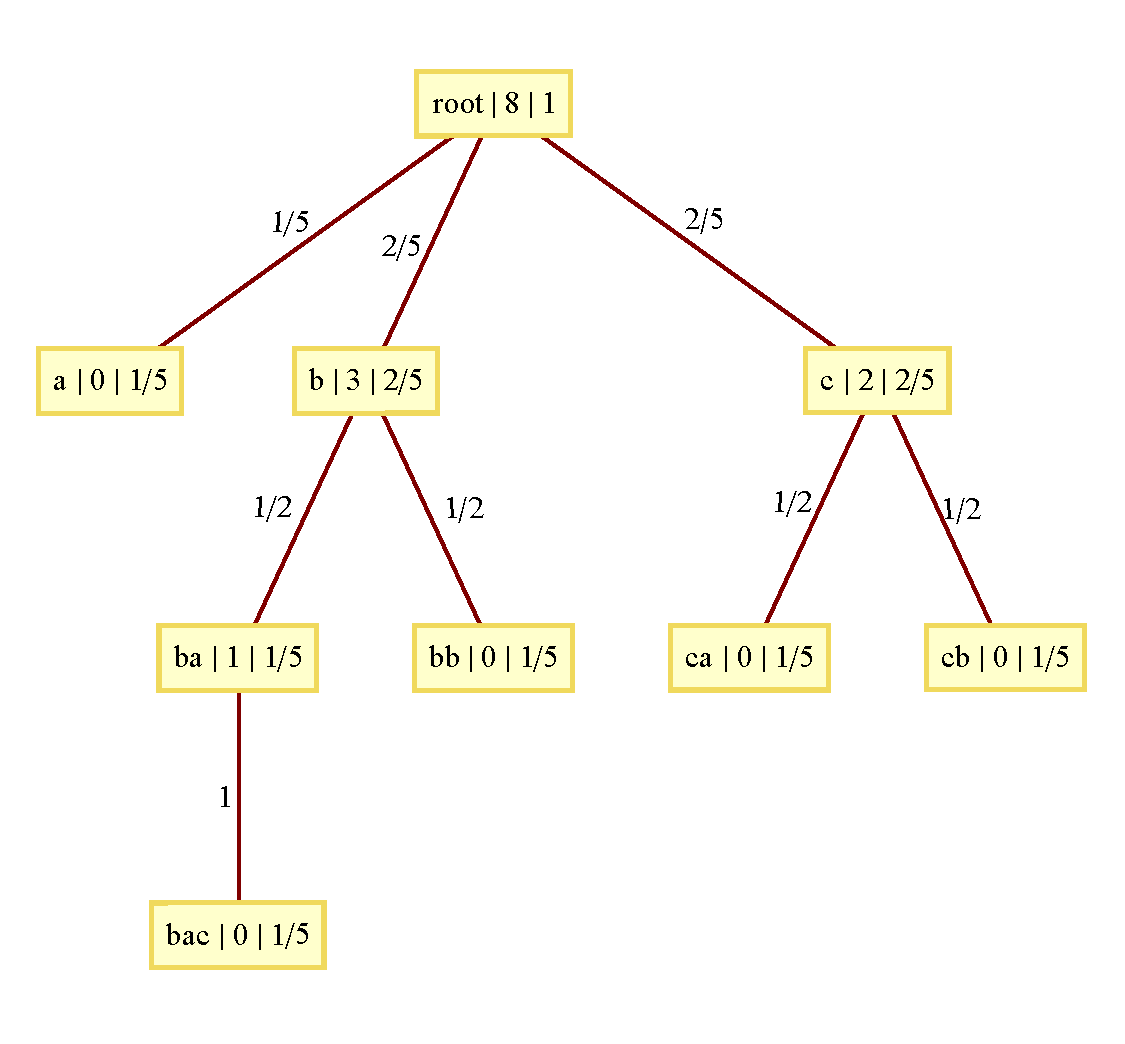
\includegraphics[width=0.40\textwidth]{sampletree.pdf}
 \caption{Sample LZ78 tree generated from the string \emph{'abbacbaccbcabb'}\label{fig:lztree}}
\end{figure} 
In \cite{Nis03}, an expanded LZ78 tree is used in order to identify the user typing on a computer keyboard. The authors suggested an expansion of the LZ78 tree seen in \cite{Lan83} by using input shifting and back-shift parsing, in order to rectify ‘noisy’ statistics caused by small training sets.

The idea to apply the LZ78 tree prediction method to malware detection was first suggested in \cite{Coh12}. Their idea included using vector quantization on packet time differences in order to predict whether unknown traffic is malicious or not - based on pre-trained sequences.


\subsection{Malware Traffic}
\label{sec:malwaretraffic}
In the past, most malware was in the form of viruses and worms, and was usually distributed physically. In recent years, with the spread of computer networks in general and the internet in particular, most malware now utilizes the internet or a local network for spreading and coordinating actions.

When a virus coordinates actions, it is known as a botnet. Such actions might include distributed attacks (like DDoS\footnote{Distributed denial of service}), personal data gathering, e-mail spam, etc. A botnet usually has a C\&C\footnote{command and control} channel that it utilizes for coordinating such attacks.
The C\&C channel is usually obscured by impersonating a well-known protocol to some extent, such as HTTP port 80, HTTPS port 443, IRC ports, etc.
The traffic generated by the malware when communicating through the C\&C channel tends to remain consistent \cite{Vil12}.

Cryptolocker is a ransomware trojan which infects Windows based PCs. Usually, the attack begins as an e-mail attachment, after which the Trojan is installed on the PC. When activated, the Trojan encrypts a selection of files on the computer using RSA public-key cryptography with the private key stored on a remote server. The user is then given an ultimatum to pay bitcoins in order to receive the decryption key. If no payment is made by the deadline, the Trojan threatens to erase the key from the server and keep all of the data encrypted.

\begin{figure}[!ht]
 \centering
 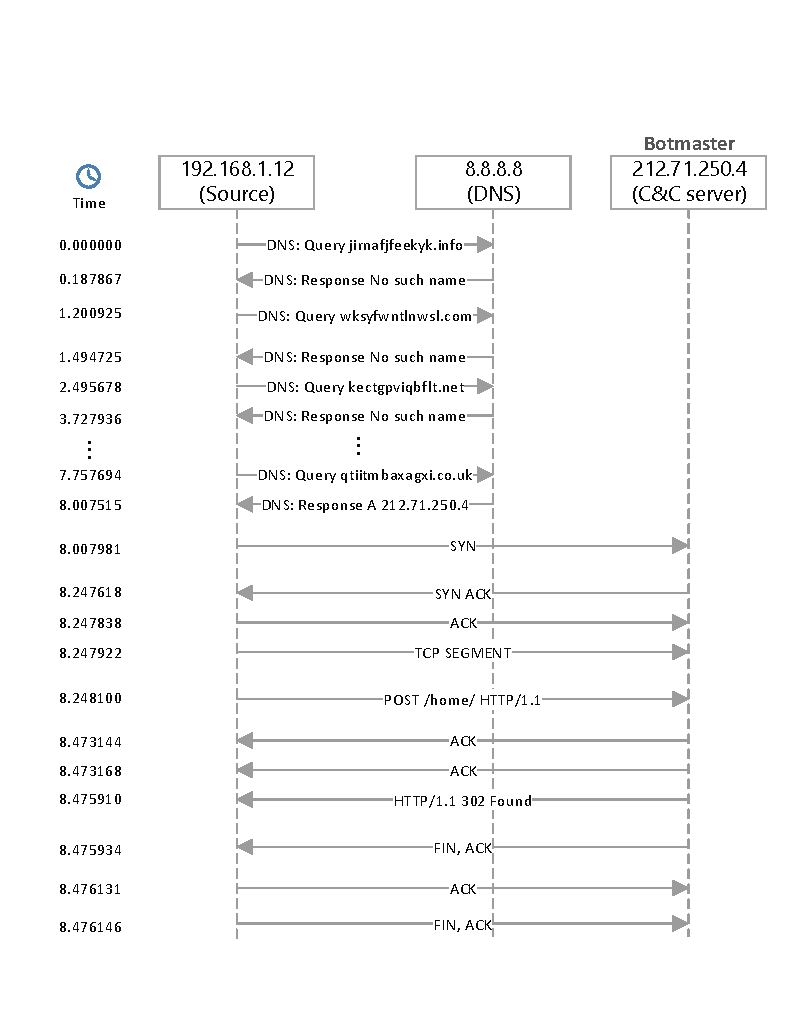
\includegraphics[width=0.5\textwidth]{fig1.pdf}
 \caption{Cryptolocker sample conversation list\label{fig:cryptolockerconv}}
\end{figure} 

Examining the Cryptolocker ransomware as a test case, an interesting network traffic profile is revealed. It first arrives via e-mail or other method. Once installed, it begins looking for a server. First, it attempts to access a hard-coded IP 184.164.136.134. If that fails, it generates a pseudo-random URL based on the time of day. This rule is known and allows the operator of the Trojan to pre-register the pseudo-random domain names \cite{EMS13}.

Once a suitable C\&C server has been found, the malware will start to communicate through regular HTTP POST requests (See figure~\ref{fig:cryptolockerconv}), albeit only as a wrapper for RSA encrypted data (See figure~\ref{fig:cryptolockerpacket}).
This behaviour is for the most part constant and was identified in several captures on different times and different machines.
\begin{figure}[!ht]
\lstset{basicstyle=\scriptsize,stringstyle=\ttfamily}
\begin{lstlisting}[frame=single,firstline=1,lastline=11]
POST /home/ HTTP/1.1
Cache-Control: no-cache
Connection: Close
Pragma: no-cache
Accept: */*
User-Agent: Mozilla/4.0 (compatible; MSIE 7.0; Windows NT 6.1; Trident/4.0; SLCC2; .NET CLR 2.0.50727; .NET CLR 3.5.30729; .NET CLR 3.0.30729; Media Center PC 6.0)
Content-Length: 192
Host: qtiitmbaxagxi.co.uk

..c/y@.
 ..`$xD2.._..dZX5..@\......e..b.B.....+.=A<"#m...q..4Ip.........C.z<{.T)-..e..A..q.......n..s...........4t.r..x.i.....y....E.]l+..c..........6..$..c...,.0..W...0f..B.<2...w}[.....f..S2
\end{lstlisting}
\caption{Cryptolocker outgoing TCP packet\label{fig:cryptolockerpacket}}
\end{figure}
\section{Identifying traffic based on the LZ78 fingerprint}
The core of our application is the LZ78 based fingerprint. Each fingerprint represents the behaviour of one malware capture.
A method for transformation of network behaviour into parsable input sequence must first be described, which in turn will be quantized using a vector-quantization clustering algorithm to be fed into the LZ78 tree creation algorithm.

\subsection{Representation via quantized packet time-difference}
The packet time difference is the time elapsed between to packet arrival/departure events in the same flow. Time difference between packets is defined as 
in (\ref{eq:timediff}) below.
\begin{equation}\label{eq:timediff}
\Delta _i \buildrel \Delta \over = {t_{i + 1}} - {t_i}
\end{equation}
Each stream of length \emph{k} is transformed into a sequence of time differences $\Delta _1, \Delta _2, ..., \Delta _k$
Because $\Delta _i \in \mathbb{R} {^ + }$  is in an infinite range, we wish to reduce the number of time differentials and smooth them over. Thus, vector quantization is performed using K-Means clustering. This enables the use of fewer symbols in the training phase which reduces variance.
\subsection{K-means clustering and K-means++ quantization scheme}
In order to quantize the packet time differences into a string parsable by the LZ78 tree-building algorithm, the K-Means++ algorithm was used.
K-Means clustering, the basis for the K-Means++ algorithm is commonly used to partition a data-set into k groups by selecting k clusters and then refining them iteratively. Since the algorithm is at its base NP-Hard, several algorithms, such as Lloyd-Max are commonly used to converge to an optimal result more quickly.

K-Means++ \cite{Art07} is an algorithm for choosing the initial seed values of the K-Means clustering algorithm first proposed in 2007 by D.~Arthur and S.~Vassilvitskii. It is an approximation algorithm for the NP-Hard K-Means problem, which avoids the sometimes poor clustering found by the Lloyd-Max algorithm.

In the program built, the input for K-Means++ is an observation vector which is all time differences seen during the extraction process described above.
The output for K-Means++ is a list of centroid values.
In order to perform quantization for each malware capture, decision boundaries must first be set. For simplicity, they are set halfway between every two centroids.
\begin{figure}[!h]
 \centering
 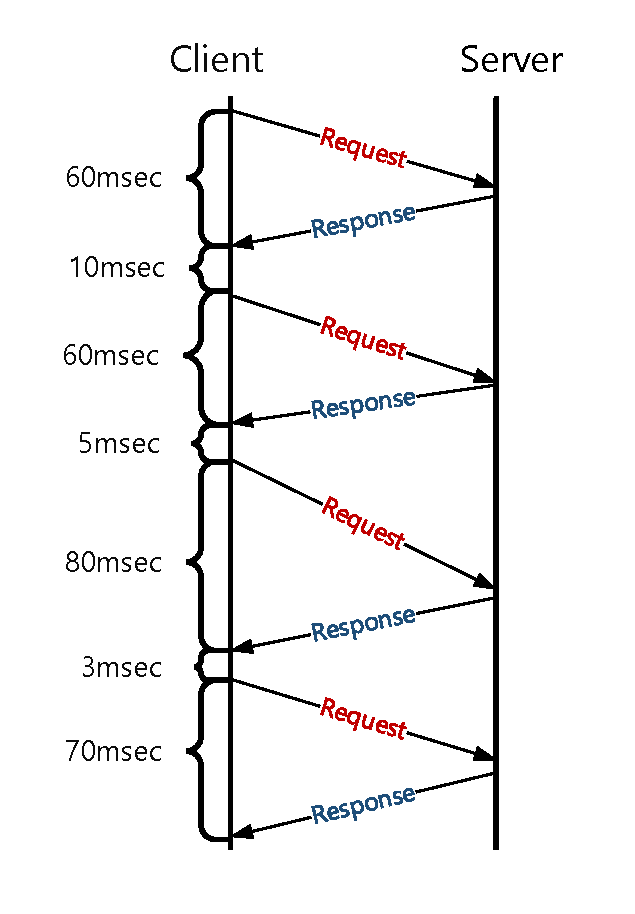
\includegraphics[width=0.2\textwidth]{fig2.pdf}
 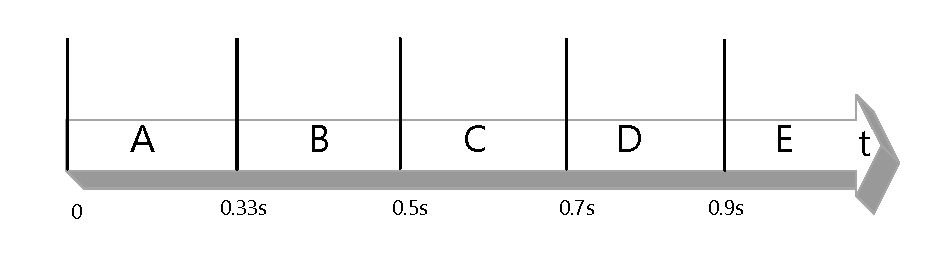
\includegraphics[width=0.4\textwidth]{fig3.pdf}
 \caption{Packet time difference quantization and letter assignment example\label{fig:packetquant}}
\end{figure} 
\subsection{Classification Methods}
\subsubsection{Smoothed KL Distance}
The \emph{Kullback--Leibler Divergence} is a metric for measuring the distance between two probability measures, defined as 
\begin{equation}\label{eq:kld}
D(P||Q) \buildrel \Delta \over = \sum\nolimits_i {\ln ({P_i}/{Q_i}) \cdot {P_i}}
\end{equation}
In the proposed algorithm, each test is composed of two probability models, consisting of discrete probabilities for the fingerprint and the raw capture data. When comparing the two trees on a node-by-node basis --- there could be a case where $Q_i=0$, causing an undefined value.
To counter this case, a modified version called \emph{Smoothed KL Distance} was devised.
The algorithm runs on two trees, where $T_{FP}$ is the fingerprint, while $T_U$ is the unknown capture.
(The trees are built as described in section \ref{section:trainingp})
\begin{algorithm}
\caption{Smoothed KL Distance}\label{kld}
\begin{algorithmic}[1]
\Procedure{SmoothedKL}{$T_{FP},T_U$}
\State $sum\gets0$
   \ForAll{Node $n_i$ in $T_{FP}$}
      \State $p_i\gets$ probability of node $n_i$
      \If{Exact matching node $m\in T_U$}
      	\State $q_i\gets$ probability of node $m$
      \Else
      	\State $q_i\gets$ probability of closest node in $T_U$ (lexicographically)
      	\State $q_i\gets q_i\cdot\varepsilon$\Comment{$\varepsilon$ is very small}
      \EndIf
   \State$sum\gets
   \log_k (p_i/q_i) \cdot {p_i}$\LONGCOMMENT{$k$ --- amount of centroids}
   \EndFor\label{euclidendwhile}
   \State \textbf{return} $sum$
\EndProcedure
\end{algorithmic}
\end{algorithm}
\subsubsection{Hamming Loss and Log Loss}
The two techniques Log loss \cite{Bis06} and Hamming loss \cite{Tso07, Ham50} are functions that represent the cost or value of an event, or an error metric.
The error metric is used due to the necessity to predict the time difference for the next packet, based on the context of the time differences seen so far.
Since discrete probabilities have already been assigned for each event, these will be the probabilities that will feature in the loss functions.
\begin{equation}\label{eq:ll}
LogLoss =  - \frac{1}{n}\sum\limits_{i = 1}^n {[{y_i}\log ({{\hat y}_i}) + (1 - {y_i})\log } (1 - {\hat y_i})]
\end{equation}
\begin{equation}\label{eq:hl}
HammingLoss({x_i},{y_i}) = \frac{1}{{\left| D \right|}}\sum\limits_{i = 1}^{\left| D \right|} {\frac{{xor({x_i},{y_i})}}{{\left| L \right|}}}
\end{equation}
Where $L$ is the number of labels, $D$ is the number of samples, $x_i$ is the prediction and $y_i$ is the ground truth.

In Log loss, the use of the log function on the probability causes extreme punishment for being confident about a wrong prediction.
In Hamming loss, any mismatch between the prediction and the real value will cause a punishment of 1.

\subsection{Program structure and algorithm}
A proof-of-concept application was built using Python due to the numerous add-on packages for parsing input files and various mathematic packages.
The program is split into two operating phases: a training phase and a testing phase.

\subsubsection{Training phase}\label{section:trainingp}
The pre-cleaned malware captures are processed to extract packet time differences.
These time differences are placed in a vector which is then quantized into a user-specified amount of values (centroids) using the K-Means++ algorithm. 
The quantized string is then used to build a LZ78 tree based on the algorithm presented previously. This represents our malware fingerprint\footnote{This action is performed for each malware capture separately}.
The fingerprints are stored in a local malware fingerprint database for easy access.
\begin{algorithm}
\caption{Training Algorithm}\label{alg:training}
\begin{algorithmic}[1]
\Procedure{Training}{}
\State ${GV}_O\gets[]; {GV}_C\gets[]$
\State ${Database}\gets[]$
   \ForAll{Capture$_i\gets$Malware captures}
   	\State \Call{AppendTo}{${GV}_O$,  [$\Delta_1,\Delta_2,...,\Delta_k$]}
   \EndFor
   \State ${GV}_C\gets$\Call{K-Means++}{${GV}_O$}

   \ForAll{Capture$_i\gets$Malware captures}
   	\State $V_i\gets\Delta_1,\Delta_2,...,\Delta_k$
   	\State Apply quantization transformation $
   	\Delta  \Rightarrow {c^*}$ where ${c^*} = \mathop {\arg \min }\limits_{{c_i}} \left| {\Delta  - {c_i}} \right|$
   	\State Map each quantized value  into a corresponding letter from the Latin alphabet ($a$,$b$,$c$,…)
   	\State ${Tree}_i\gets$\Call{LZ78 Tree Generation}{ [$c_1$,$c_2$,$c_3$,...] as a string}
    \State Append to ${Database}\gets{Tree}_i$ \label{alg:training:append_db}
   \EndFor
   \State \textbf{return} $Database$
\EndProcedure
\end{algorithmic}
\end{algorithm}
\subsubsection{Testing phase}
In the testing phase, an unknown capture is to be assigned a score in comparison with our fingerprint database. The lower the score, the better the match.

A process identical to the training phase is performed on the unknown capture to be tested, with the exception of Algorithm~\ref{alg:training} stage~\ref{alg:training:append_db} --- the capture is not placed in the database.
 
The unknown capture is then compared against the known malware database fingerprint by fingerprint, using three different algorithms – Smoothed KL-Distance, Log Loss and Hamming Loss.

Each of these algorithms returns a numerical value for each pair of fingerprints. These values will be used to classify the capture as malware or malware free.
\section{Datasets and Experimental Setup}
\subsection{Gathering data}
\subsubsection{Malware dataset}
Wireshark captures containing known malware were used, captured by a third-party using sandboxed computers.
The captures were identified by the third-party, and contained many varied traffic interspersed: UDP, TCP, HTTP, POP3 and ICMP to name a few.

Captures from malware that communicates to remote machines via WAN were used.
The captures used include malwares named Renovator (1 capture),  Cryptolocker (10 captures), Bladabindi (3 captures), DarkComet (2 captures) and Hesperbor (3 captures).

Some of the malware tested attempted to obscure itself as standard HTTP traffic (as described with Cryptolocker in section \ref{sec:malwaretraffic}), while some access other TCP ports.
\subsubsection{Control dataset}
The control dataset includes some background data and website access traffic.
The traffic was captured using Wireshark on standard Windows 7 personal computers. Supplemental captures were obtained from readily available Wireshark capture repositories.
Captures include standard HTTP traffic, SMTP, IRC, Spotify, IMAP and NNTP (7 captures).
\subsection{Filtering the captures}
Filtering irrelevant entries in the traffic captures required onerous non-automated work.
First, all traffic inside the LAN was removed. WAN IPs were cross-referecned with malware research websites in order to discover if any IPs have already been 'incriminated'.
Similar actions were performed on DNS requests to reveal malicious URLs.
All traffic to non-incriminated URL and IPs was then removed, leaving behind the core behaviour of the malware.

\subsection{Experimental results}
The test setup included training on the malware dataset and control dataset.
The number of centroids was set to 25 for all tests.

Raw, uncleaned captures of malware and other background traffic was collected, being captured on different occasions and different machines. These captures will be tested and verified against the fingerprint database created during training.

The results shown only includes the {\em Smoothed KL distance} method. The other methods examined did not yield sufficiently certain results.

Table \ref{table:testresults} specifies results for comparing an unknown capture versus the fingerprint database using the {\em Smoothed KL Distance method}.

A lower result indicates that the distance between the unknown capture and the fingerprint is smaller, meaning a better match.

Examining the \emph{Cryptolocker $\alpha$} test, the best matches are against other captures of Cryptolocker (See Table \ref{table:testresults} below), with the exception of Cryptolocker $\beta$ which exhibited slightly different behaviour.

The \emph{Hesperbor} malware capture shows much better results when compared to other versions of the malware, with a distance metric smaller than $1$.
For the other fingerprints, the distance metric is much larger ($>3.0$).

Empirically, it was established that results below $3.0$ represent a good match. In future works, this parameter can be used as a classifier rule for deciding if a capture contains malware traffic.

\begin{figure}[!h]
 \centering
 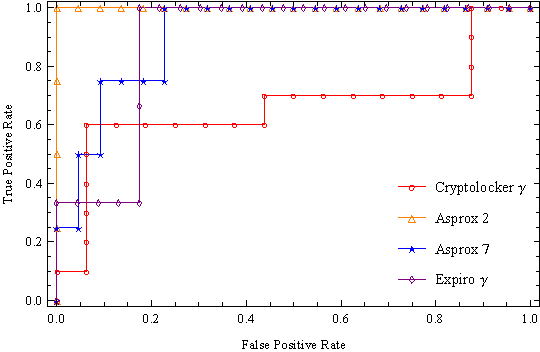
\includegraphics[width=0.4\textwidth]{roc1.pdf}
 \caption{Characteristic ROC for various captures \label{fig:roc1}}
\end{figure} 

\begin{figure}[!h]
 \centering
 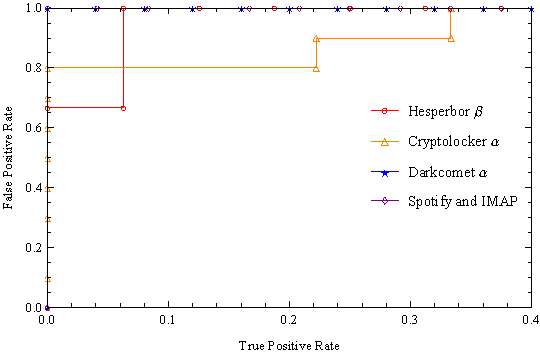
\includegraphics[width=0.4\textwidth]{roc2.pdf}
 \caption{Zoom in on Figure \ref{fig:roc1} \label{fig:roc2}}
\end{figure} 

\begin{table}[!ht]
% increase  table row spacing, adjust to taste
\renewcommand{\arraystretch}{1.15}
% if using array.sty, it might be a good idea to tweak the value of
% \extrarowheight as needed to properly center the text within the cells
\caption{Test results for various raw captures}
\label{table:testresults}

% Some packages, such as MDW tools, offer better commands for making tables
% than the plain LaTeX2e tabular which is used here.
\begin{tabular}{|p{1.56cm}|p{1.4cm}|p{1.3cm}|p{1.2cm}|p{1.4cm}|}
\hline
Fingerprint& \textbf{Cryptlocker $\alpha$ (raw)}&\textbf{Hesperbor (raw)}&\textbf{DozmotD}&\textbf{Spotify and IMAP}\\
\hline
Telnet&9.43&8.17&11.05&9.58\\
\hline
Spotify&11.78&15.25&17.73&\textbf{4.26}\\
\hline
SMTP&4.90 &10.09&8.78&10.06\\
\hline
NNTP&12.08&9.37&13.83&7.75\\
\hline
IRC&27.07&21.01&23.90&16.58\\
\hline
HTTP, JPEG &18.98 &8.12&18.25&11.64\\
\hline
Bitorrent &5.9 &9.11&9.96&5.52\\
\hline
Renovator $\gamma$ 1 &5.02&4.31&5.80&4.65\\
\hline
Hesperbor $\beta$ 3 &3.39&1.40&4.67&6.80\\
\hline
Hesperbor $\beta$ 2 &3.47&1.69&4.98&5.45\\
\hline
Hesperbor $\beta$ 1 &3.32&\textbf{0.44}&4.62&5.90\\
\hline
Darkcomet $\alpha$ 2 &11.11&12.18&13.44&13.96\\
\hline
Darkcomet $\alpha$ 1 & 11.11&12.19&13.41&13.94\\
\hline
Cryptolocker $\gamma$ 2 &0.45&8.1&5.09&9.07\\
\hline
Cryptolocker $\gamma$ 1&0.39&6.22&5.95&9.93\\
\hline
Cryptolocker $\beta$ 4&2.23&23.73&21.50&23.16\\
\hline
Cryptolocker $\beta$ 3 &5.07&34.79&31.52&33.80\\
\hline
Cryptolocker $\beta$ 2&1.54&13.26&12.60&13.97\\
\hline
Cryptolocker $\beta$ 1&1.87&32.58&29.60&30.95\\
\hline
Cryptolocker $\alpha$ 4&1.15&6.07&5.74&9.79\\
\hline
Cryptolocker $\alpha$ 3&0.48&5.51&6.58&8.05\\
\hline
Cryptolocker $\alpha$ 2&\textbf{0.31}&7.11&8.37&9.85\\
\hline
Cryptolocker $\alpha$ 1&1.54&3.25&\textbf{2.91}&7.25\\
\hline
Bladabindi $\alpha$ 3&3.18&5.41&6.60&6.56\\
\hline
Bladabindi $\alpha$ 2&4.29&6.67&9.12&9.60\\
\hline
Bladabindi $\alpha$ 1&3.66&3.61&6.38&6.74\\
\hline
\end{tabular}
\\  
  
Notes:
\begin{itemize}
\item \textbf{Bold} text marks best match.
\item All raw captures differ from training captures.
\item The DozmotD malware underwent no training at all.
\end{itemize}
\end{table}

% needed in second column of first page if using \IEEEpubid
%\IEEEpubidadjcol

% An example of a floating figure using the graphicx package.
% Note that \label must occur AFTER (or within) \caption.
% For figures, \caption should occur after the \includegraphics.
% Note that IEEEtran v1.7 and later has special internal code that
% is designed to preserve the operation of \label within \caption
% even when the captionsoff option is in effect. However, because
% of issues like this, it may be the safest practice to put all your
% \label just after \caption rather than within \caption{}.
%
% Reminder: the "draftcls" or "draftclsnofoot", not "draft", class
% option should be used if it is desired that the figures are to be
% displayed while in draft mode.
%
%\begin{figure}[!t]
%\centering
%\includegraphics[width=2.5in]{myfigure}
% where an .eps filename suffix will be assumed under latex, 
% and a .pdf suffix will be assumed for pdflatex; or what has been declared
% via \DeclareGraphicsExtensions.
%\caption{Simulation Results.}
%\label{fig_sim}
%\end{figure}

% Note that IEEE typically puts floats only at the top, even when this
% results in a large percentage of a column being occupied by floats.
% However, the Computer Society has been known to put floats at the bottom.


% An example of a double column floating figure using two subfigures.
% (The subfig.sty package must be loaded for this to work.)
% The subfigure \label commands are set within each subfloat command,
% and the \label for the overall figure must come after \caption.
% \hfil is used as a separator to get equal spacing.
% Watch out that the combined width of all the subfigures on a 
% line do not exceed the text width or a line break will occur.
%
%\begin{figure*}[!t]
%\centering
%\subfloat[Case I]{\includegraphics[width=2.5in]{box}%
%\label{fig_first_case}}
%\hfil
%\subfloat[Case II]{\includegraphics[width=2.5in]{box}%
%\label{fig_second_case}}
%\caption{Simulation results.}
%\label{fig_sim}
%\end{figure*}
%
% Note that often IEEE papers with subfigures do not employ subfigure
% captions (using the optional argument to \subfloat[]), but instead will
% reference/describe all of them (a), (b), etc., within the main caption.


% An example of a floating table. Note that, for IEEE style tables, the 
% \caption command should come BEFORE the table. Table text will default to
% \footnotesize as IEEE normally uses this smaller font for tables.
% The \label must come after \caption as always.
%
%\begin{table}[!t]
%% increase table row spacing, adjust to taste
%\renewcommand{\arraystretch}{1.3}
% if using array.sty, it might be a good idea to tweak the value of
% \extrarowheight as needed to properly center the text within the cells
%\caption{An Example of a Table}
%\label{table_example}
%\centering
%% Some packages, such as MDW tools, offer better commands for making tables
%% than the plain LaTeX2e tabular which is used here.
%\begin{tabular}{|c||c|}
%\hline
%One&Two\\
%\hline
%Three&Four\\
%\hline
%\end{tabular}
%\end{table}


% Note that IEEE does not put floats in the very first column - or typically
% anywhere on the first page for that matter. Also, in-text middle ("here")
% positioning is not used. Most IEEE journals use top floats exclusively.
% However, Computer Society journals sometimes do use bottom floats - bear
% this in mind when choosing appropriate optional arguments for the
% figure/table environments.
% Note that, LaTeX2e, unlike IEEE journals, places footnotes above bottom
% floats. This can be corrected via the \fnbelowfloat command of the
% stfloats package.



\section{Conclusion}
The conclusion goes here.





% if have a single appendix:
%\appendix[Proof of the Zonklar Equations]
% or
%\appendix  % for no appendix heading
% do not use \section anymore after \appendix, only \section*
% is possibly needed

% use appendices with more than one appendix
% then use \section to start each appendix
% you must declare a \section before using any
% \subsection or using \label (\appendices by itself
% starts a section numbered zero.)
%


\appendices

% you can choose not to have a title for an appendix
% if you want by leaving the argument blank
\section{}
Appendix 1


% use section* for acknowledgement
\ifCLASSOPTIONcompsoc
  % The Computer Society usually uses the plural form
  \section*{Acknowledgments}
\else
  % regular IEEE prefers the singular form
  \section*{Acknowledgment}
\fi


The authors would like to thank...


% Can use something like this to put references on a page
% by themselves when using endfloat and the captionsoff option.
\ifCLASSOPTIONcaptionsoff
  \newpage
\fi



% trigger a \newpage just before the given reference
% number - used to balance the columns on the last page
% adjust value as needed - may need to be readjusted if
% the document is modified later
%\IEEEtriggeratref{8}
% The "triggered" command can be changed if desired:
%\IEEEtriggercmd{\enlargethispage{-5in}}

% references section

% can use a bibliography generated by BibTeX as a .bbl file
% BibTeX documentation can be easily obtained at:
% http://www.ctan.org/tex-archive/biblio/bibtex/contrib/doc/
% The IEEEtran BibTeX style support page is at:
% http://www.michaelshell.org/tex/ieeetran/bibtex/
%\bibliographystyle{IEEEtran}
% argument is your BibTeX string definitions and bibliography database(s)
%\bibliography{IEEEabrv,../bib/paper}
%
% <OR> manually copy in the resultant .bbl file
% set second argument of \begin to the number of references
% (used to reserve space for the reference number labels box)
\begin{thebibliography}{10}

\bibitem{Lem78}
Avraham~Lempel and Jacob~Ziv.
\newblock Compression of individual sequences via variable-rate coding.
\newblock {\em IEEE Transmissions on Information Theory}, page 530–536, September 1978.

\bibitem{MFe92}
Meir~Feder and Neri Merhav and Michael~Gutman.
\newblock Universal prediction of individual sequences.
\newblock {\em IEEE Transactions on Information Theory}, 38(4):1258–1270, July 1992.

\bibitem{Nis03}
Mordechai~Nisenson and Ido Yariv and Ran El-Yaniv and Ron~Meir.
\newblock Towards Behaviometric Security Systems: Learning to Identify a Typist.
\newblock {\em Knowledge Discovery in Databases: PKDD 2003, Lecture Notes in Computer Science}, 2838:363–374, 2003.

\bibitem{Lan83}
Jr~Langdon G.G.
\newblock A note on the Ziv - Lempel model for compressing individual sequences (Corresp.).
\newblock {\em IEEE Transactions on Information Theory}, 29(2):284–287, 1983.

\bibitem{Coh12}
Asaf~Cohen and Shlomi Dolev and Niv Gilboa and Guy~Leshem.
\newblock Anomaly Detection, Dependence Analysis and.
\newblock Technical Report, Ben Gurion University of the Negev, Beersheba,, 2012.

\bibitem{Vil12}
Nart~Villeneuve and James~Bennett.
\newblock Detecting APT Activity with Network Traffic Analysis.
\newblock 2012.

\bibitem{EMS13}
EMSISoft~Blog.
\newblock CryptoLocker - a new ransomware variant
\newblock Available: {\em http://blog.emsisoft.com/2013/09/10/cryptolocker-a-new-ransomware-variant/}, [Accessed 16 August 2014]

\bibitem{Art07}
David~Arthur and Sergei~Vassilvitskii.
\newblock k-means+: The advantages of careful seeding.
\newblock {\em Proceedings of the eighteens annual ACM-SIAM symposium on Discrete algorithms}, page 1027–1035, 2007.

\bibitem{Kul51}
Solomon~Kullback and Richard~Leibler.
\newblock On Information and Sufficiency.
\newblock {\em The Annals of Mathematical Statistics}, 22(1):79–86, 1951.

\bibitem{Bis06}
Christopher~M Bishop.
\newblock {\em Pattern Recognition and Machine Learning}.
\newblock Springer, Cambridge, UK, 2006.

\bibitem{Tso07}
Grigorios~Tsoumakas and Ioannis~Katakis.
\newblock Multi-label classification: An overview
\newblock {\em International Journal of Data Warehousing and Mining}, 3(3):1-13, 2007.

\bibitem{Ham50}
Richard~W Hamming.
\newblock Error detecting and error correcting codes.
\newblock {\em Bell Systems technical journal}, 29(2):147–160, 1950.


\end{thebibliography}

% biography section
% 
% If you have an EPS/PDF photo (graphicx package needed) extra braces are
% needed around the contents of the optional argument to biography to prevent
% the LaTeX parser from getting confused when it sees the complicated
% \includegraphics command within an optional argument. (You could create
% your own custom macro containing the \includegraphics command to make things
% simpler here.)
%\begin{IEEEbiography}[{\includegraphics[width=1in,height=1.25in,clip,keepaspectratio]{mshell}}]{Michael Shell}
% or if you just want to reserve a space for a photo:

\begin{IEEEbiography}{Name}
Biography text here.
\end{IEEEbiography}

% if you will not have a photo at all:
\begin{IEEEbiographynophoto}{Name}
Biography text here.
\end{IEEEbiographynophoto}

% insert where needed to balance the two columns on the last page with
% biographies
%\newpage

% You can push biographies down or up by placing
% a \vfill before or after them. The appropriate
% use of \vfill depends on what kind of text is
% on the last page and whether or not the columns
% are being equalized.

%\vfill

% Can be used to pull up biographies so that the bottom of the last one
% is flush with the other column.
%\enlargethispage{-5in}



% that's all folks
\end{document}


